\documentclass[12pt,a4paper]{article}
\usepackage[utf8]{inputenc}
\usepackage[french]{babel}
\usepackage[T1]{fontenc}
\usepackage{amsmath}
\usepackage{amsfonts}
\usepackage{amssymb}
\usepackage{makeidx}
\usepackage{multicol}
\usepackage{svg}
\usepackage{lipsum}
\usepackage{capt-of}
\usepackage{verbatimbox}
\usepackage[left=2.5cm,top=2cm,right=2.5cm]{geometry}
\begin{document}
\begin{titlepage}
\begin{center}
\textbf{\textsc{UNIVERSIT\'E LIBRE DE BRUXELLES}}\\
\textbf{\textsc{Faculté des Sciences}}\\
\textbf{\textsc{Département d'Informatique}}
\vfill{}\vfill{}
\begin{center}{\Huge Implémentation d'une formulation étendue pour la conception d'un réseau de distribution d'électricité}\end{center}{\Huge \par}
\begin{center}{\large Frantzen Christian}\end{center}{\Huge \par}
\vfill{}\vfill{}
\begin{flushleft}{\large \textbf{Superviseur : Bernard Fortz}}\hfill{}\end{flushleft}{\large\par}
\vfill{}\vfill{}\enlargethispage{3cm}
\textbf{Année académique 2015~-~2016}
\end{center}
\end{titlepage}
\tableofcontents
\pagebreak
%\begin{abstract}
%\lipsum[1]
%\end{abstract}
\begin{multicols}{2}
\section{Introduction}
La transition énergétique pose beaucoup de nouveaux défis pour l'industrie. Souvent de grandes centrales de production d'électricité sont remplacées par plusieurs centrales plus petites. Ceci nécessite un changement important dans la configuration du réseau. La configuration d'un réseau de distribution d'électricité a un impact important sur des paramètres physiques comme perte d'énergie de de tensionainsi que la charge des points-clés d'un réseau comme les transformateurs. Pour prendre en compte tous ces facteurs mais en gardant un niveau d'abstraction élevé, Rossi et al \cite{Rossi} introduisent un paramètre de distance maximale $D_{max}$. On considère qu'un client alloué à un fournisseur à une distance inférieure à $D_{max}$ n'est pas soumis à des phénomènes de perte d'énergie ou de tension trop importants.\newline \indent
Le but des algorithmes présentés dans leur article est de maximiser la marge minimale des différentes sources du réseau. La marge d'une source est la différence entre sa capacité de production d'énergie et la demande totale des clients connectés à cette source.\newline \indent
Avoir une grande marge une caractéristique de robustesse d'un réseau face à des augmentations spontanée de la demande.
\section{Approche}
\subsection{Définition du problème}
Pour résoudre le problème, on représente le réseau par un graphe non-dirigé $G(V,E)$, où $V$ est l'ensemble des sommets et $E$ est l'ensembles des arrêtes. L'ensemble des sommets $V$ est l'union des ensembles disjoints des clients  $V_{c}$ et des fournisseurs $V_{f}$. L'ensemble $E$ représente les différents connexions avec interrupteur entre les sommets. $n_{f}=|V_{f}| $ est le nombre de fournisseurs dans le réseau et $n_{c}=|V_{c}| $ est le nombre de clients. Chaque sommet $j$ dans $V_{f}$ a un poids $pow_{j}$ qui représente sa capacité maximale de production d'énergie. Chaque sommet $i$ dans $V_{c}$ a un poids $dem_{i}$ qui représente a demande d'énergie.La distance minimale entre 2 sommets $i$ et $j$ dans $G$ est donnée par $d_{i,j}$ est représente un nombre de sauts. Comme $G$ est non-dirigé, $d_{i,j}=d_{j,i} \forall (i,j) \in V \times V$. L'ensemble des clients pour lesquelles la distance minimale entre eux et le fournisseur $j$ est inférieure à $D_{max}$ est noté $N_{j} \forall j \in V_{f}$. $N_{j}$ est l'ensemble des clients qui peuvent potentiellement être connectés au fournisseur $j$. S'il existe un client qui ne se retrouve dans aucun ensemble $N_{j}$, la résolution est infaisable.
\subsection{Contraintes}
Une configuration est faisable si elle respecte les contraintes suivantes :
\begin{enumerate}
\item Contrainte de demande : La capacité d'un fournisseur doit être suffisante pour satisfaire la demande des clients auxquels il est connecté.
\item Contrainte de connectivité : pour des raisons techniques, deux fournisseurs ne doivent pas être connectés entre eux, ce que implique que chaque client doit être connecté à exactement un fournisseur. Chaque sous-graph de $G$ doit être non-cyclique.
\item Contrainte de distance : Pour minimiser les phénomènes de perte d'énergie et de tension, les clients ne doivent pas être alloués à des fournisseurs à une distance supérieure à $D_{max}$.   
\end{enumerate}
\subsection{Conditions de faisabilité}
Pour que la résolution du problème soit faisable, il existe 2 conditions nécessaire pour garantir la faisabilité :
\begin{itemize}
\item La somme des capacités des fournisseurs doit satisfaire la demande totale des clients : \begin{equation*}
\sum_{j \in V_{f}}{pow_{j}}  = \sum_{i \in V_{c}}{dem_{i}}
\end{equation*}
\item Pour chaque client il existe un ou plusieurs fournisseurs à une distance inférieure ou égale à $D_{max}$ :
\begin{equation*}
\forall i \in V_{c} :  \exists j \in V_{f} \mid dist(j,i) \leq D_{max}
\end{equation*}
\end{itemize}
Si c'est deux conditions ne sont pas satisfaite, on peut démontrer que la résolution du problème est infaisable.\\
Pour rendre la résolution plus facile, dans notre configuration, on attribue à chaque fournisseur la capacité de satisfaire tous les clients : 
\begin{equation*}
\forall j \in V_{f} : pow_{j}=\sum_{i \in V_{c}}{dem_{i}}.
\end{equation*}
\section{Méthode implémentée}
\subsection{Formulation orientée sommets}
Dans l'article, il y a 2 types de formulations utilisées pour le problème. Une qui ne prend en compte que les sommets du graphe et ne décide que si un client $i$ est alloué ou pas à un fournisseur $j$ et l'autre formulation ne prend en compte que l'état des différentes arrêtes du graphe et décide s'il y a un flux de courant électrique qui la traverse ou pas.\newline\indent
Dans ce travail, on se concentre sur la formulation avec les sommets, ainsi, on a les variables de décision suivantes : $\forall (i,j) \in V_{c}\times V_{f}$, $ x_{i,j}$ est mise à 1 si et seulement si le client $i$ est alloué au fournisseur $j$, sinon $x_{i,j}=0$. Les contraintes de la formulation sont décrites ici :
\begin{equation}\label{eq:Obj}
Maximiser \ M_{min}
\end{equation}
\begin{equation}\label{eq:powDem}
pow -\sum_{i \in N{j}}{x_{i,j}dem_{i}} \geq M_{min} \ \forall j \in V_{f}
\end{equation}
\begin{equation}\label{eq:oneFeeder}
\sum_{i \in V_{c}}{x_{i,j}}=1 \ \forall j \in V_{f}
\end{equation}
\begin{equation}\label{eq:N_j}
x_{i,j}=0 \ \ \forall j \in V_{f},\forall i \notin N_{j}
\end{equation}
\begin{equation}
\begin{aligned}\label{eq:connect}
&\mbox{Les clients alloués au fournisseurs j} \\ 
&\mbox{ forment un component connecté } \\
& \forall j \in V_{f}
\end{aligned}
\end{equation}
\begin{equation}\label{eq:dist}
\begin{aligned}
&\mbox{La distance d'un client i à son}\\ 
&\mbox{fournisseur est inférieure ou égale } \\
& \mbox{à } D_{max} \ \forall i \in V_{c}
\end{aligned}
\end{equation}
\begin{equation}\label{eq:0_1}
x_{i,j} \in \{0,1 \} \ \forall (i,j) \in V_{c}\times V_{f}
\end{equation}
\begin{equation}\label{eq:Mmin_0}
M_{min}\geq 0
\end{equation}
\eqref{eq:Obj} est la fonction objectif: maximiser la marge minimale pour tous les fournisseurs. \eqref{eq:powDem} définit la marge minimale pour tous les fournisseurs. La contrainte \eqref{eq:oneFeeder} assure que chaque client soit alloué à 1 fournisseur et \eqref{eq:N_j} assure qu'un client ne soit pas alloué à un fournisseur situé à une distance supérieure à $D_{max}$. Les contraintes \eqref{eq:connect} et \eqref{eq:dist} sont difficile à enforcer, ils seront expliquer en détail dans la section à suivre. La contrainte \eqref{eq:0_1} assure l'intégralité de solution et \eqref{eq:Mmin_0} la non-négativité.\newline \indent
Le modèle de programmation linéaire principal se compose des contraintes \eqref{eq:Obj}-\eqref{eq:N_j}, \eqref{eq:0_1} ,\eqref{eq:Mmin_0} ainsi que des \textit{layer inequalities} (inégalités des couches), qui seront expliqués plus tard. Les \textit{layer inequalities} n'aident pas seulement à atteindre la solution optimale, mais aussi à converger plus rapidement.
\subsection{Layer inequalities}
Les layer inequalities restreignent le problème principal pour qu'il n'assume pas de solutions qui ne seront jamais bonnes. Les layer inequalities fonctionnen comme suit : les clients se trouvant à une distance $\lambda$ au fournisseur $j$ dans le graphe appartiennent à la couche $L_{j,\lambda}$. Ainsi $\forall j \in V_{f}$ et $\forall \lambda \in \{1,...,D_{max} \}$, tout client $i \in L_{j,\lambda + 1}$ peut être alloué au fournisseur $j$ si et seulement si il y a au moins un client $k \in L_{j,\lambda}$ qui lui aussi est alloué au fournisseur $j$. Cette contrainte peut s'écrire : 
\begin{align*}
x_{i,j} \leq \sum_{k \in L_{j,\lambda} }{x_{k,j}} \forall i \in L_{j,\lambda +1},\\ \forall \lambda \in \{ 1,...,D_{max}-1 \}, \forall j \in V_{f}
\end{align*}
Ces inégalités enforcent des conditions nécessaires pour la connectivité des la solution ainsi que partiellement prenant en compte les exigences de distance. Elles peuvent être rendues plus stricte en ajoutant la condition que pour tout client $i$ dans $L_{j,\lambda +1}$, seul des clients $k$ dans $L_{j,\lambda}$ qui se trouvent à une distance plus petite ou égale à $D_{max}-\lambda$ de $i$ avec tous les clients alloués sur le chemin entre $i$ et $k$ se trouvant à une distance strictement plus grande que $\lambda$ de $j$ peuvent assurer la connectivité de la solution.S'il n'y a pas de chemin entre $k$ et $i$ d'une longueur inférieur ou égale à $D_{max}-\lambda$, alors le client n'est pas aidant pour connecter $i$ à $j$. De plus, si sur les chemins entre $k$ et $i$ se trouvent un client $v \neq i$ pour lequel la distance à $j$ est plus petite ou égale à $\lambda$, alors le client $i$ peut être connecté à j à travers $v$ et on n'a pas besoin du client $k$.\newline \indent
Pour construire les layer inequalities, on a besoin de deux ensembles, $R_{k,j}$ et $P_{i,j}$. Soit k un client dans $L_{j,\lambda}$. L'ensemble des clients pour lesquels la distance jusqu'à $j$ est strictement plus grande que $\lambda$ et pour lesquels la distance jusqu'à $k$ est plus petite ou égale à $D_{max}-\lambda$ est noté $R_{k,j}$. Cet ensemble peut être considéré comme l'ensemble des clients qui peuvent être connectés à $j$ à travers $k$ on satisfaisant la contrainte de distance. Soit $i$ un client dans la couche $L_{j,\lambda +1}$. L'ensemble des prédécesseur potentiels dans $L_{j,\lambda}$ est noté $P_{i,j}$. Ainsi au moins un client dans $P_{i,j}$ doit être alloué au fournisseur $j$ pour que $i$ soit connecté à $j$.\newline\indent
Plus précisément :
\begin{align*}
&R_{k,j} = \{ v | \lambda < d_{v,j} \wedge d_{v,k}\leq D_{max}-\lambda \} \\ 
&\forall k \in L_{j,\lambda}, \forall \lambda \in \{ 1,...,D_{max}-1 \}, \forall j \in V_{f}\\
&P_{i,j} = \{ k \in L_{j,\lambda} \ i \in R_{k,j} \} \forall i \in L_{j,\lambda +1}, \\ 
&  \forall \lambda \in \{ 1,...,D_{max}-1 \}, \forall j \in V_{f}
\end{align*}
Ainsi les inégalités des couches sont définies comme suit : 
\begin{equation}\label{eq:layers}
\begin{aligned}
x_{i,j} \leq \sum_{k\in P_{i,j}}{x_{k,j}} \forall i \in L_{j,\lambda +1}, \\ \forall \lambda \in \{ 1,...,D_{max}-1 \}, \forall j \in V_{f}
\end{aligned}
\end{equation}
Comme tout client n'apparaît qu'au plus une fois dans une couche $L_{j,\lambda}$ pour tous les fournisseurs $j \in V_{f}$,le nombre d'inégalités des couches est au plus $n_{c}\times n_{f}$.
\subsection{Méthode des plans sécants}
\subsubsection*{Coupes de connectivité}
Les inégalités des couches sont efficace mais il ne suffisent pas pour enforcer la connectivité de la solution, c'est la raison pourquoi des coupes de connectivité sont ajoutées au problème principal. \newline \indent
Chaque fois que le problème principal est résolu, le component connecté associé avec le fournisseur $j$, noté $CC_{j}$ est construit pour tout $j$ dans $V_{f}$. L'ensemble des clients qui sont alloués au fournisseur $j$ mais qui ne sont pas dans $CC_{j}$ est noté $O_{j}$.\newline \indent
Si $O_{j}$ est non vide alors les clients alloué au fournisseur $j$ ne forment pas un component connecté, la solution n'est pas admissible et une coupe de connectivité est requise. Soit $CS_{j}$ l'ensemble des clients adjacent à $CC_{j}$ mais qui sont alloués à un fournisseur différent de $j$. $CS_{j}$ peut être appelé ensemble de coupe (\textit{cut set}) : enlever ses clients de $G$ isolerait les clients dans $CC_{j}$ du reste du graphe, particulièrement de $O_{j}$. Ainsi, pour que les clients dans $O_{j}$ soient atteignables depuis $j$, au moins un client dans $CS_{j}$ doit être alloué au fournisseur $j$. On peut l'écrire comme suit : 
\begin{equation}\label{eq:connect1}
\sum_{i \in O_{j}}{x_{i,j}} \leq |O_{j}|\sum_{i \in CS_{j}}{x_{i,j}} \ \forall j \in V_{f}
\end{equation}
L'inégalité \eqref{eq:connect1} représente une coupe de connectivité. En théorie, une solution connectée peut être atteinte en intégrant les coupes de connectivité au modèle principal, or ce serait inefficace et requerrait un grand nombre d'itérations. Ainsi, à la place de générer une seule coupe de connectivité pour le fournisseur $j$, le nombre de coupes de connectivité à ajouter au problème principal est égal au nombre de composants connectés dans $O_{j}$. Ceci requiert la construction de $C_{j}$, l'ensemble de tous les composants connectés dans $O_{j}$. Soient $CC$ un composant connecté dans $C_{j}$ et $CS$ l'ensemble des clients adjacents à $CC$  qui ont un fournisseur différent de $j$. Pour qu'un client dans $CC$ puissent être connecté au fournisseur $j$, au moins un client dans $CS$ doit aussi être alloué à $j$. La version simplifié d'une coupe de connectivité peut être écrite comme suit :
\begin{align*}
&x_{i,j} \leq |O_{j}|\sum_{k \in CS}{x_{k,j}} \ \forall i \in CC, \\ 
&\forall CC \in C_{j}, \forall j \in V_{f}\\ 
\end{align*}
Pour diminuer le nombre de coupes de connectivité, une seule coupe de connectivité est générée pour chaque component connecté $CC$ dans $O_{j}$, pour tout $j \in V_{f}$. D'abord, un client $i_{cc} \in CC$ se trouvant à une distance de $j$ qui est minimale entre tous les clients $i \in CC$ est choisi aléatoirement. Ensuite tous les clients $k$ dans $CS$ tels que $d_{k,j}+d_{k,i_{cc}}>D_{max}$ sont enlevés de $CS$. Ils ne sont pas utiles pour connecter $i_{cc}$ à $CC_{j}$ dans l'itération suivante de l'algorithme des plans sécants. Plus précisément, la coupe de connectivité associée à $CC$ est
\begin{equation}
\begin{aligned}
x_{i,j} \leq  \sum_{\substack{k \in CS \\d_{k,j}+d_{k,i_{cc}}\leq D_{max}}}{x_{k,j}} \\  
\forall CC \in C_{j}, \forall j \in V_{f}\\ 
\end{aligned}
\end{equation}
\subsubsection*{Coupes de distance}
Pour tout fournisseur $j \in V_{f}$, les contraintes de distance ne sont vérifiées que lorsque $j$ et ses clients forment un component connecté. Il peut paraître étonnant que cette contrainte puisse être violée si on n'alloue que des clients de $N_{j}$ à $j$, or une situation peut arriver où des clients se trouvant sur les plus court chemins entre les clients alloués à $j$ et $j$ sont alloués à un fournisseur différent et peuvent ainsi bloquer l'utilisation du plus court chemin, ce qui allonge les chemins restants et rend possible le dépassage de la longueur maximale $D_{max}$.\newline \indent
Comme les contraintes de distance ne sont vérifiées que lorsque les contraintes de connectivité sont satisfaites pour un fournisseur $j$, $O_{j}$ est vide mais l'ensemble $CS_{j}$ est construit quand même. Soit $F_{j}$ l'ensemble des clients alloués à $j$ à une distance de $D_{max}+1$ de $j$ dans la solution courante.\newline \indent
Une version simplifée des coupes de distance dit que pour diminuer la distance entre $j$ et un client $i$ dans $F_{j}$, au moins un client dans $CS_{j}$ doit être alloué à $j$:
\begin{equation*}
x_{i,j} \leq \sum_{k \in CS_{j}}{x_{k,j}} \ \forall i \in F_{j}, \forall j \in V_{f}
\end{equation*}
À nouveau, on diminue le nombre de coupe de distance:
\begin{equation}
\begin{aligned}
x_{i,j} \leq \sum_{\substack{k \in CS \\d_{k,j}+d_{k,i}\leq D_{max}}}{x_{k,j}} \ \forall i \in F_{j}, \forall j \in V_{f}
\end{aligned}
\end{equation}

\subsection{Déroulement de l'algorithme}
La figure \ref{fig:algo} (à la fin du document) présente le déroulement de l'algorithme de la méthode des plans sécants. Comme déjà mentionné, le modèle de programmation linéaire principal se compose des contraintes \eqref{eq:Obj}-\eqref{eq:N_j} et \eqref{eq:0_1} -\eqref{eq:layers}. Après chaque résolution du problème principal on vérifie si on doit ajouter des contraintes supplémentaires au problème, si non cela veut dire que la solution courante satisfait toutes les contraintes et elle est finale.
\section{Résultats expérimentaux}
\subsection{Génération de graphes}
Les graphes générés pour tester l'algorithme sont rectangulaires. Un fournisseur se trouve dans chaque n-ième ligne du graphe, leur position dans la ligne étant déterminée aléatoirement. Le reste du graphe est rempli avec des clients aléatoires. La demande d'un client est un nombre entier entre 1 et 100. Chaque client est connecté à ses voisins horizontaux et verticaux.
\begingroup
    \centering
    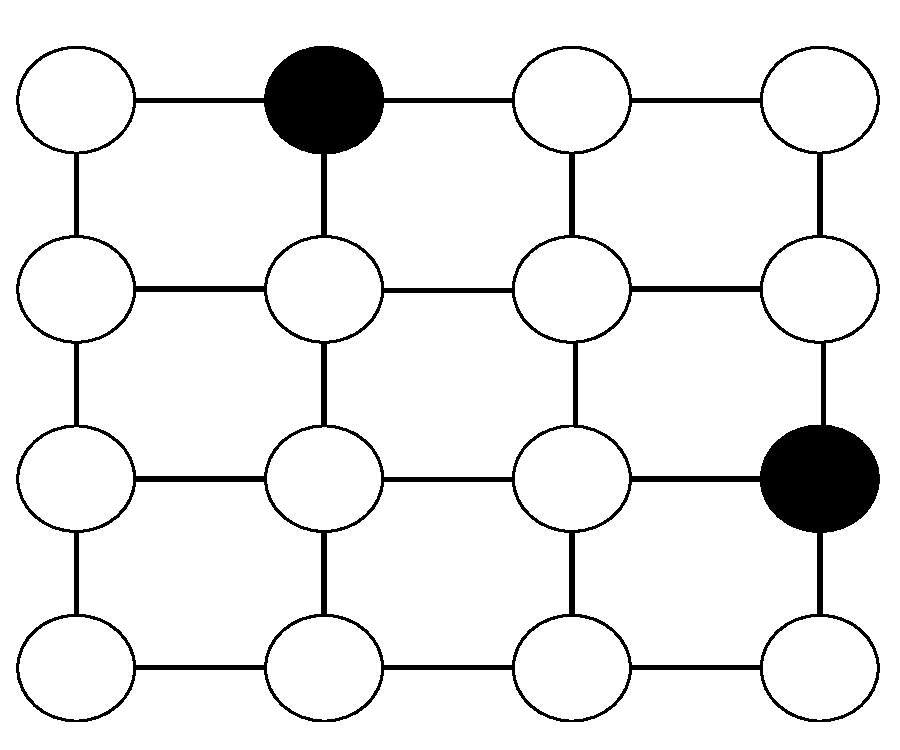
\includegraphics[width=\linewidth]{graph4x4.pdf}
    \captionof{figure}{Représentation d'un graphe 4$\times$4. Les sommets en noirs sont les fournisseurs }\label{fig:algo}
\endgroup
\subsection{Résultats}
Les expériences ont toutes été réalisées sur Ubuntu 14.04 LTS tournant dans VMware Workstation 10 tournant sur Windows 10, le processeur étant un Intel Core 4500U à 1.8 GHz avec 4GB de RAM pour la VM et 8GB pour l'ordinateur de base. Le solveur de programmation linéaire utilisé est CPLEX d'IBM.
\addvbuffer[12pt]{\begin{tabular}{|c|c|c|c|c|c|c|c|}
\hline 
dim & n &$n_{f}$ & $n_{c}$ & deg & temps & iter & inst \\ 
\hline 
5x5 & 2 & 3 & 22 & 3.2 & 7.48 & 19.3 & 10  \\ 
\hline 
6x6 & 2 & 3 & 33 & 3.33 & 92.13 & 63.18  & 11\\ 
\hline 
7x7 & 2 & 4 & 45 & 3.43 & • & • & 0 \\ 
\hline
\end{tabular}}
La colonne \textit{dim} indique les dimensions du graphe. La colonne \textit{n} spécifie la valeur du pas de lignes lors de création du graphe pour l'insertion d'un fournisseur. Les colonnes $n_{f}$ et $n_{c}$ indiquent évidemment le nombre de fournisseurs et de clients dans le graphe. La colonne \textit{deg} donne le degré moyen des sommets dans le graphe. La colonne \textit{temps} donne la durée d'exécution moyenne du programme en secondes CPU, \textit{iter} indique le nombre d'itérations moyen de l'algorithme. Le nombre d'instances de graphes considéré pour déterminé les valeurs est donné dans la colonne \textit{inst}.
\subsection{Discussion}
On voit très bien l'augmentation du temps de calcul en n'ajoutant que 11 clients au graphe de 4$\times$4 pour arriver aux graphes 5$\times$5, le facteur d'augmentation est plus grand que 10.
\section{Conclusion et perspectives}


\end{multicols}
\begingroup
    \centering
    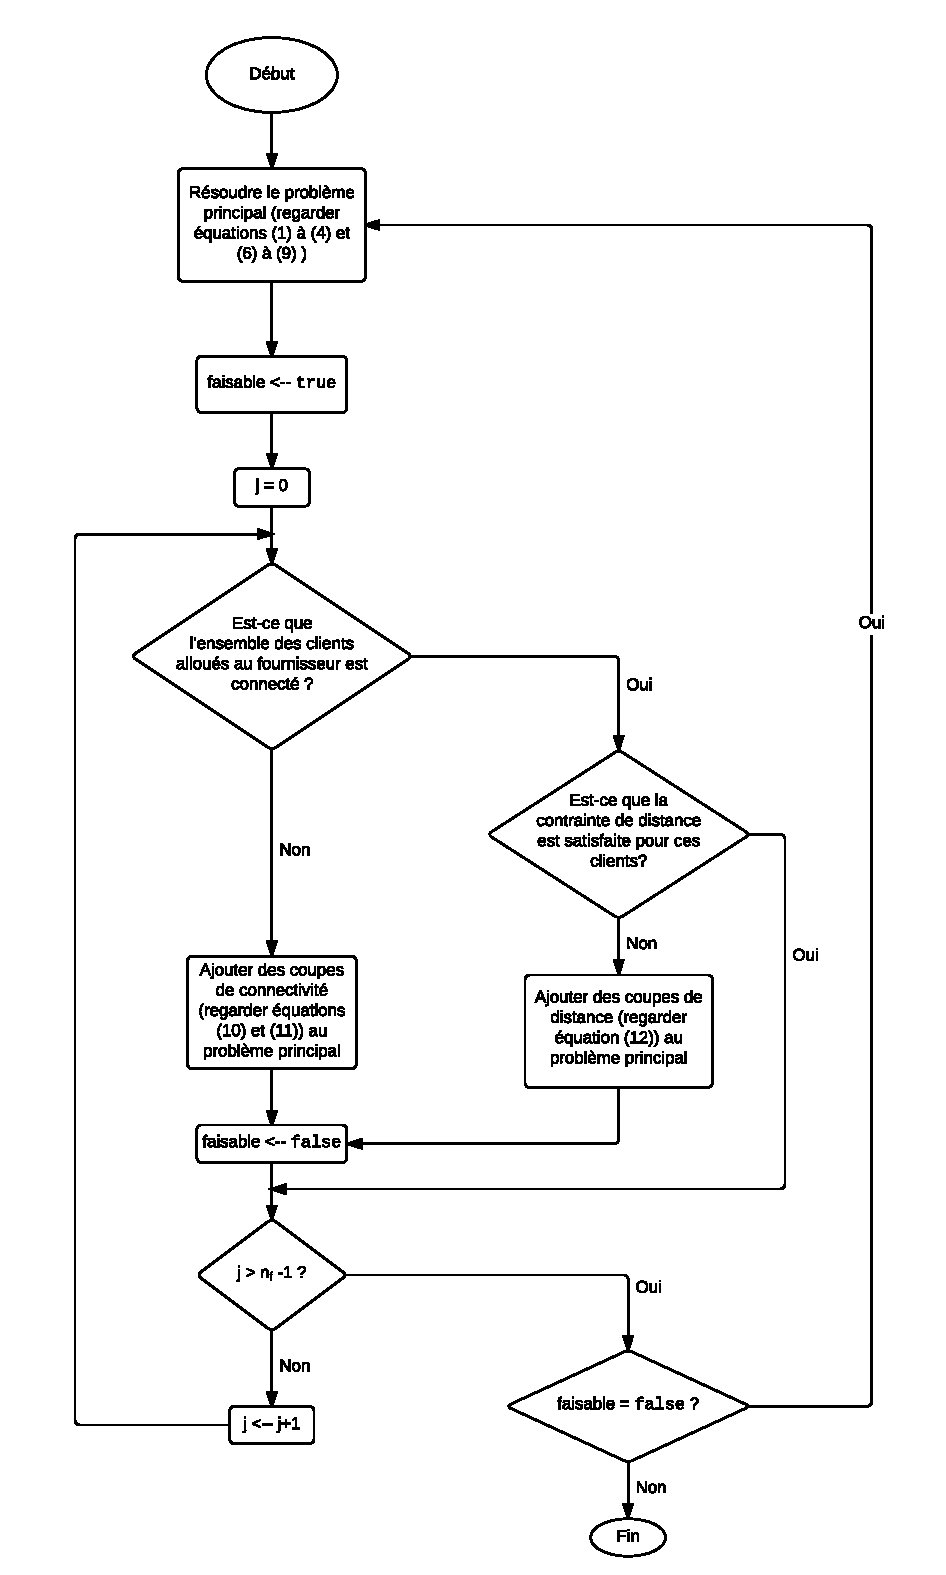
\includegraphics[height=23cm]{flowChartAlgo.pdf}
    \captionof{figure}{Flowchart du \textit{cutting plane} algorithme}\label{fig:algo}
\endgroup
\begin{multicols}{2}
\bibliographystyle{apalike}

\begin{thebibliography}{20}
\bibitem{Rossi}
André Rossi, Alexis Aubry, Mireille Jacomino, Connectivity-and-hop-constrained design of electricity distribution networks,  \textit{European Journal of Operational Research}, 218 2012, 48-57
\end{thebibliography}
\end{multicols}
\end{document}